\documentclass[Main]{subfiles}
\begin{document} 
\begin{otherlanguage*}{italian}

%	\chapter*{Acknowledgement  \markboth{}{}}
	\chapter*{Ringraziamenti  \markboth{}{}}
	\it
		E' molto sentito da parte mia ringraziare tutti coloro che mi hanno aiutato nella realizzazione di questa Tesi e che mi sono stati vicini, con enorme pazienza, durante questi lunghi anni di studio.
		\vspace{1mm} \\
		Per primi voglio ringraziare i miei \emph{mentori}, Claudio Dappiaggi e Franco Magri, che mi hanno fatto conoscere e amare la Fisica-Matematica, e il professor Livio Pizzocchero che mi ha reso possibile seguire questa mia passione.% avermi indicato la giusta via e avermi permesso di seguirla.
		\vspace{1mm} \\
		Ringrazio i miei \emph{mecenati}, Pappio e Mamma, che mi hanno supportato in ogni aspetto possibile della vita: affettivo, emotivo, intellettivo e, soprattutto per quanto riguarda l'università, economico.
		\vspace{1mm} \\
		Ringrazio la mia \emph{musa}, Giusy, per aver sempre creduto in me, facendomi tirare fuori tutto il mio meglio... e sopportandomi tutte quelle volte che il mio meglio non è bastato.
		\vspace{1mm} \\
		Ringrazio le mie sorelle Serena, Irene e Silvia, i miei nipotini Daniele, Martina, Giulia, Diego e Gaia, i miei cugini Gianluca, Diego, Alberto, Andrea ed Elena e tutto il resto della mia grande famiglia per non aver mai smesso di farmi sentermi amato.
		\vspace{1mm} \\
		Per ultimi, ma non meno importanti, voglio ringraziare tutti i miei buoni amici che sono stati un sostegno indispensabile durante questi 10 anni di università:
	
			\begin{figure}[h!]
				\centering
  				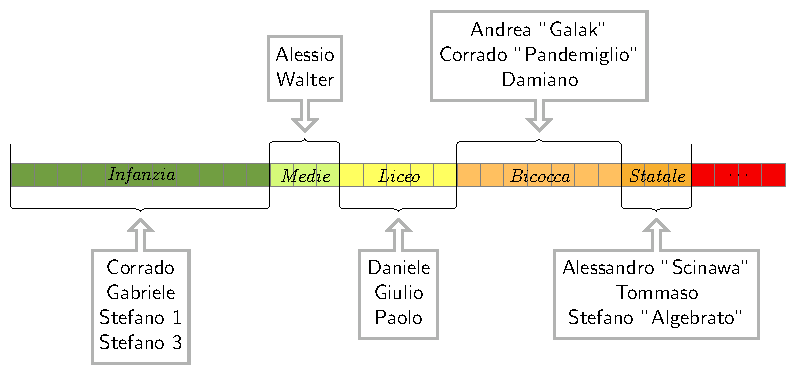
\includegraphics[width=0.8\textwidth]{Fun/TimeLine}					
			\end{figure}	
	
	
\end{otherlanguage*}
\end{document}
 	
% 			Amici:\\
%			Infanzia: Corrado A., Gabriele, Stefano 1, Stefano 3\\
% 			Medie: Travani, Walter\\
%			Liceo: Coto, Red, Saffo \\
% 			Uni: Damiano, Galak, Pandemiglio, Tommaso,Scin\\
% 			Popolo di Lcm